\chapter{Implementation}\label{chp:impl}

The key features of the MCDTP implementation (MCDTPi) are its use of the modular and asynchronous programming paradigms. This is further discussed in this section.

\section{Why F\#?}

The F\# language, like C\#, can run atop the .NET Core Framework \cite{Leijen2009}\cite{syme2011f}. F\# was chosen over C\# because of the features that are exclusive to F\#. The key aspect of F\# is the embedded domain specific language (EDSL) \cite{syme2011f}. The EDSL in F\# adds a component to F\# called ``computation expression'' that provides an abstraction to using features like asynchrony \cite{syme2011f}. The F\# compiler allows for custom computation expressions to be defined as will be shown in Section \ref{sec:api}.

Consider the following synchronous code:

\begin{lstlisting}[caption=Synchronous F\# Example,label={lst:sync}]
let child() =
  System.Threading.Thread.Sleep(1000)
  printfn "Hello from child!"

let parent() =
  printfn "Parent calling child..."
  child()

parent()
\end{lstlisting}

The asynchronous equivalent is:

\begin{lstlisting}[caption=Asynchronous F\# Example,label={lst:async}]
let asyncChild =
  async {
    do! Async.Sleep(1000)
    printfn "Hello from child!"
  }

let asyncParent =
  async {
    printfn "Parent calling child..."
    do! asyncChild
  }

Async.RunSynchronously asyncParent
\end{lstlisting}

The transformation from synchronous code to asynchronous code is surprisingly straight forward thanks to the compiler, which is further discussed here \cite{syme2011f}. The ease of composing asynchronous tasks helps simplify constructing an asynchronous workflow, which is further discussed in Section \ref{sec:async-arch}.

\section{Modular Architecture}\label{sec:mod-arch}

The modular approach to programming breaks a large codebase into smaller chunks called modules based on some criteria \cite{Microsystems2007}. Typically modules address a specific problem. Modules are also agnostic to outside code. This enables the ability to swap out modules for others. The implementation of MCDTP uses a modular architecture to help manage the complexity the codebase.

\begin{figure}[ht]
\centering
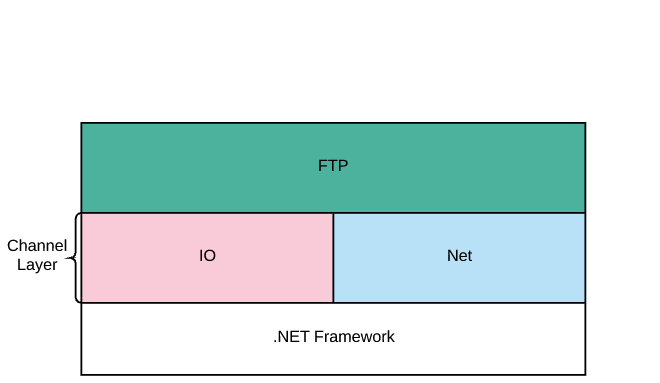
\includegraphics[scale=0.4]{MCDTPArchitecture}
\caption{The architecture of the MCDTP implementation}
\label{fig:mcdtp-arch}
\end{figure}

The top module is an $FTP$ module and depends on an $IO$ module and a $Net$ module. The .NET Framework is the base module of MCDTPi that uses the cross-platform variant called .NET Core Framework \cite{netCore10}. MCDTPi was built using version 1.0.3 of the .NET Core Framework \cite{netCore103}. Its source code can be found here \cite{netCore103Src}. The MCDTPi modules, and their respective submodules, will be reviewed in the order of dependency.

\subsection{Helper Modules}

There are two micro-modules that are used thoughout all modules and submodules in MCDTPi. The $Logging$ and $Utility$ modules, as seen in Figure \ref{fig:mcdtp-hm}, contain helper code that is commonly used throughout MCDTPi. The $Logging$ module was created to manage console and log file outputs for easier debugging. This module provides two configurable loggers, a console logger and a network logger. The console logger is a general purpose logger that writes trace messages and debug messages to the console to provide real-time diagnostics of MCDTPi. The network logger logs events pertaining to Socket I/O operations like packet transmission or reception as well as packet loss events to a file for each channel. Both loggers support log level configurations to filter out messages below a certain priority.

\begin{figure}[ht]
\centering
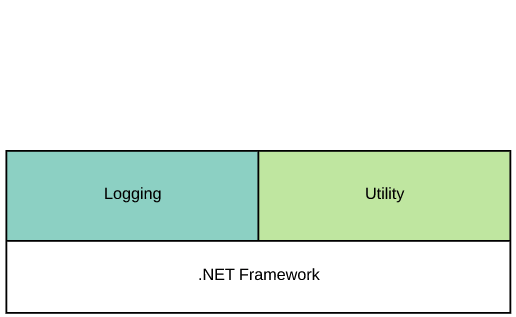
\includegraphics[scale=0.4]{MCDTPHelperModules}
\caption{MCDTP Helper Modules}
\label{fig:mcdtp-hm}
\end{figure}

The $Utility$ module provides code for type conversion, which is mostly used for serialization and deserialization purposes, as well as code for wrapping a function with a semaphor type data structure. This module is used mostly to provide abstractions to reocurring code snippets found throughout MCDTPi.

\subsection{IO Module}

The $IO$ module is one of the major modules to MCDTPi. The module handles all I/O related operations, except for socket I/O, see Section \ref{sec:net} for more details. This module is composed of three submodules, as seen in Figure \ref{fig:mcdtp-io-arch}.

\begin{figure}[ht]
\centering
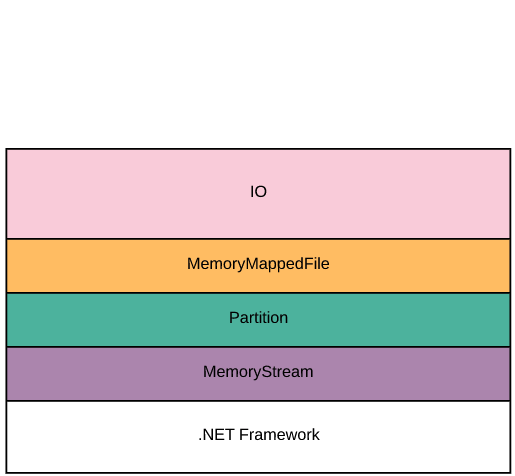
\includegraphics[scale=0.4]{MCDTPIOArchitecture}
\caption{MCDTP IO Architecture}
\label{fig:mcdtp-io-arch}
\end{figure}

\subsubsection{Memory Stream Sub-Module}

The $MemoryStream$ submodule is largely based on the $MemoryStream$ data structure found in the .NET Framework. The difference is that this submodule provides an unbounded buffer. The .NET Framework data structure has an upper bound on how much data can be written to the $MemoryStream$, which is $\frac{2^{32}}{2} - 1$. This can result in a performance issue because it would restrict the amount of data that can be held in memory to 2GB. This is fine for low end machines, but many machines have 8GB or more of memory. The imposed upper bound needed to be mitigated through the use of a custom $MemoryStream$.

Instead of using a single byte array as the underlying container, MCDTPi uses a linked list of byte arrays to provide an unbounded container. Bytes are written to the end of the stream just like the original data structure; however, when a byte array fills up, an empty byte array is added to the end of the list so that more bytes can be added to the stream. As bytes are being read from a stream, the first array shrinks until it is empty, then it is removed from the list, and the next byte array will be consumed. Though this stream is unbounded, its API uses bounded arrays as arguments and return values. The context in which this submodule will be used means that it should accept a bounded array as argument for writing to stream as well as returning a bounded array for read operations.

\subsubsection{Partition Sub-Module}

The $Partition$ submodule is actually a submodule to $MemoryMappedFile$ and uses $MemoryStream$ as a dependency. This submodule is used to read and write part of a file. The ``part'', or partition, has a $PartitionHandler$. This data structure is used to manager a file pointer within that part of the file. The $PartitionHandle$ keeps track of the state of the buffer and file pointer to ensure that any asynchronous I/O task, involving either the $MemoryStream$ or disk, do not overlap. This submodule is configurable with respect to how frequent a disk I/O operation should happen, whether it is read only or write only, and the console logger configuration it should use. Specifications like where the partition begins in the file and how large the partition is can be configured as well; however, it is highly recommended that those properties be set by the parent module $MemoryMappedFile$.

Additionally, $Partition$ handles special writes for data snippets in one of two ways. The initial method is to try and amend the buffer. The position in buffer is determined by the position in file the data snippet belongs to. The position in file is offset by the position of the beginning of the buffer. This gives how far into the buffer the snippet needs to be written. If the beginning of the buffer is positioned after the data snippet in file, then a write needs to happen that involves temporarily moving the file pointer to write the data snippet to disk and returning the file pointer back to its previous position.

\subsubsection{Memory Mapped File Sub-Module}

The $MemoryMappedFile$ submodule is the top submodule in the $IO$ module. This submodule is the parent of $Partition$. It is inspired by the .NET Framework data structure of the same name. However, the difference lies in the functionality. Like the original data structure, $MemoryMappedFile$ is used to store large portions of a file in memory from different locations within the file. This submodule treats these portions as ``partitions'', whereas the data structure treats them as ``views''. A view in the data structure is a portion of a file that is loaded into memory. A partition is a portion of a file that has a dedicated file pointer and is only partially loaded into memory, which would be the view of the partition.

Though the differences seem marginal, the major reason for creating this submodule was the ability to shift the view to a new position in file. The original data structure does not provide such functionality. Instead, to move a view would require creating a whole new view. Views would also need to be smaller to minimize the footprint on memory required to hold at most two views in memory. Smaller views would mean more disk I/O operations to try and mitigate any interruption that may occur by either depleting the buffer representing the view, or filling buffer to capacity. This is why a custom submodule was constructed. To provide the ability to have a sliding view for reducing complexity of managing data in memory.

This functionality is offloaded to the child submodule $Partition$ since it is an action that happens to a partition of a file. $MemoryMappedFile$, instead, handles partitioning a file equally so that each partition is roughly of equal size. The configurable properties of a $MemoryMappedFile$ are the file name, used to identify a file to read or a new file to write to; the number of partitions to create, though it is recommended that $FTP$ set this; the $Partition$ configuration to use; and whether this file should be opened as read only or write only.

\subsection{Net Module}\label{sec:net}

Another core module to MCDTPi is the $Net$ module. This module handles network related actions, such as application level packet managing, parsing and composing raw data, and performing socket I/O operations. Like the $IO$ module, $Net$ is comprised of multiple submodules, as shown in Figure \ref{fig:mcdtp-net-arch}. Notice that the submodules are side-by-side instead of stacked like the $IO$ module, indicating that the modules are independent of one another.

\begin{figure}[ht]
\centering
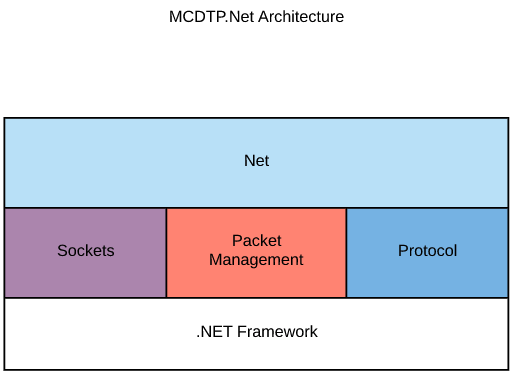
\includegraphics[scale=0.4]{MCDTPNetArchitecture}
\caption{MCDTP Net Architecture}
\label{fig:mcdtp-net-arch}
\end{figure}

\subsubsection{Protocol Sub-Module}

The Application Layer protocol that MCDTP defines is a very simplistic protocol. However, the implementation is a little more complex and thus, to help with maintainablility, MCDTPi has split the protocol into two modules and the $Protocol$ submodule is one of them. Divvying up the protocol like this means that any future work that changes the messages being sent and received only effects this submodule. The raw data that is sent or received is handled by this submodule. The $Protocol$ submodule parses and composes raw data, or more commonly known as deserialize and serialize, sometimes called ``SerDe'', a data structure, respectively. Both of TCP and UDP packet structures discussed in Section \ref{sec:proto-des} are handles by this submodule. $Protocol$ uses $Utility$ to convert raw bytes to more understandable primitive types. $Logging$ is also a dependency to provide output for error messaging so that when a message does not parse or compose correctly, the invalid input can be fetched for analysis if there is the need. The API of this submodule will be discussed in Section \ref{sec:api}.

\subsubsection{Sockets Sub-Module}

All socket operations are housed in the $Sockets$ submodule. A configurable type class called $SocketHandle$ that wraps a socket is provided by this submodule. This type class is capable of performing pre- and post- socket I/O operations. This is more for compatability with $Protocol$. The pre- and post-operations are configurable so that any message handling service can be performed when raw data is sent or received. Note, sending data is an asynchronous operation. Firstly, it uses the provided asynchronous send function provided by .NET Framework. Secondly, it queues messages if an asynchronous operation is running. The receive operation is asynchronous as well thanks to the .NET Fremework, however, queueing receive requests is not supported. $SocketHandle$ is used for both TCP and UDP sockets and can be configured to use either protocol. Currently, IPv4 is the only supported version of the Internet Protocol. Section \ref{sec:api} will provide a code snippet on how the $Sockets$ module is used.

\subsubsection{Packet Management Sub-Module}\label{sec:pm-sm}

The second submodule that implements the remainder of the UDP component of MCDTP is $PacketManagement$. This submodule has many working parts, as will be discussed. $PacketManagement$ is used to manage UDP packets. From the server's perspective, data is loaded from a source and converted to packets using $Protocol$. Packets are buffered and made accessible through a function call. When enough packets have been depleted, another batch is loaded. When there are no more packets to be loaded, the server buffers the final packet as per the design of MCDTP data transmission phase. The final packet is submitted to the front of the retransmit queue to ensure the client receives that packet.

It is worth noting that the $PacketManagement$ module does not know the origin of the data it loads. This module does not know the size of the data source either. This agnostic behavior enables this module and the parent module, $Net$, to interface with any data source provided that the end of the source is indicated by no data being loaded.

When a packet is lost, the server gets a report that a packet, identified by a sequence number, has been lost. When $PacketManagement$ gets this report, the sequence number is submitted to a queue for processing, and, if the retransmit processor has not been initialized, it is setup to run on a configured interval. As reports come in, the retransmit processor will take a report and fetch the data from source and queue it up for retransmission. $PacketManagement$ is preconfigured to have 40 packets available for retransmission and send only five at a time, which is mostly to not obstruct the flow of the data transmission phase. The interval the retransmit processor executes is configurable. When the time is due to run the retansmit processor, it will copy up to five packets and push them on to the front of the main queue. During this time, the processor will also check to see if the retransmit queue needs to be reloaded. If so, any reports that are pending will be processed and moved to the retransmit queue. If there is no data to load and the rtransmit queue is empty, the retransmit processor will uninitialize itself, otherwise, it reinitializes itself for another interval. Any acknowledged packets are removed from either queue.

On the client, packet loss is detected by gaps in the packet sequence numbers. Sequence numbers increase by the size of a packet. This is reliable because all packets are of the same size with the exception being the last packet. Thus, when a sequence number increases by more than the size of a packet, a packet has been dropped. This detection occurs during the flush event. The flush event occurs when the buffer size exceeds a configured threshold. As a packet loss is detected, missing data is temporarily filled in with null values to ensure data remain in its correct position and a report list is compiled of all packets that have been lost. This list is sent over TCP to ensure the server knows which packets need to be retransmitted. When a packet is recovered, an acknowledgement is sent to the server. The data in the recovered packet is submitted to $Partition$ for handling.

\subsection{FTP Module}

The $FTP$ module is the top module of MCDTPi. It interacts with the lower modules and helps $Net$ interact with $IO$, since they are sibling modules, by providing callback functions that can be used by either $Sockets$ or $PacketManagement$. $FTP$ manages the data channels, and ensures that a data channel on the server matches a data channel on the client by pairing the start position of each partition to each port used by a UDP socket in ascending order--each channel is identified by the port. This is reliable because as per MCDTP design, ports are exchanged during the handshake. This module also handles all TCP communication and performs the associated action for a TCP packet. For instance, a packet loss report is directly handled by $FTP$ and forwards the report to the channel with the matching port identification. $FTP$ also prepares the $MemoryMappedFile$ submodule on both client and server. When both hosts are ready, $FTP$ initiates the transmission process. While this is running, $FTP$ exposes a state that represents the state of all channels. When all channels have succeeded, $FTP$ assumes the succeeded state. This module is configurable and propagates the configurations for the lower modules onward.

\section{Asynchrony}\label{sec:async-arch}

Asynchrony is used extensively throughout MCDTPi. It is used not only at the implementation level, but at an architectural level as well so that sibling modules that exchange messages back and forth have minimal impact on one another's performance.

For instance, when a UDP packet is received on the client, it gets processed by $Sockets$ and $Protocol$ and is submitted to $PacketManagement$. $PacketManagement$ decides if this packet will trigger a flush event or not. If it does not, the packet is simply added to the buffer. If it does, $PacketManagement$ asynchronously flushes the buffer by submitting the received data to $Partition$. If this action triggers a flush event within $Partition$, an internal asynchronous task will flush data to disk. When the $Socket$ module submits data to $PacketManagement$ module, the $Socket$ module is not blocked by $PacketManagement$ while it decides what to do. The $Socket$ module can return to receiving packets. The same interaction exists between $PacketManagement$ and $Partition$. This data flow from $Socket$ to $Partition$ is on the client. The server's data flow is in the opposite direction, from $Partition$ to $Socket$, but has the same non-blocking characteristic.

\section{API}\label{sec:api}

F\# provides the ability to create computation expressions like the $async$ keyword in Listing \ref{lst:async}. MCDTPi takes advantage of this to provide a concise API for generating configurations used to configure the modules and submodules. The following code examples illustrate how straight forward it is to set up an MCDTPi instance on a server and client.

\begin{lstlisting}[caption=Server Example]
// create logger configurations
let console =
  loggerConfig {
    useConsole
    loggerId "Simple Console"
    // use the highest log level to maximize log data
    logLevel LogLevel.Info
  }
let network =
  loggerConfig {
    networkOnly
    loggerId "Simple Network"
    // use the highest log level to maximize log data
    logLevel LogLevel.Info
  }

// create socket configurations
let tcp = socketHandle { useTcp }
let udp = socketHandle { useUdp }

// create partition configuration
let partitionConfig =
  partition {
    // when buffer falls below 50MB, load another 50MB
    replenishThreshold (50 * 1000 * 1000)
    isReadOnly
    attachLogger console
  }

// create memoryMappedFile configuration
let mmfConfig =
  mmf {
    usePartitionConfig partitionConfig
    handleFile fileName
    isReadOnly
  }

// create ftp configuration
let ftpConfig =
  ftp {
    serverMode
    useConsole console
    monitorNetwork network
    configureUdp udp
    configureTcp tcp
    useParser Tcp.Parser.tryParse
    useComposer Tcp.Composer.tryCompose
    channelCount 4 // use 4 data channels
  }

let session = Ftp.acceptNewSessionFromConfig ftpConfig
session.BeginHandshakeAsServer()

\end{lstlisting}

\vskip 0.8in

\begin{lstlisting}[caption=Client Example]
// create logger configurations
let console =
  loggerConfig {
    useConsole
    loggerId "Simple Console"
    // use the highest log level to maximize log data
    logLevel LogLevel.Info
  }
let network =
  loggerConfig {
    networkOnly
    loggerId "Simple Network"
    // use the highest log level to maximize log data
    logLevel LogLevel.Info
  }

// create socket configurations
let tcp = socketHandle { useTcp }
let udp = socketHandle { useUdp }

// create partition configuration
let partitionConfig =
  partition {
    // when buffer exceeds 50MB, flush to disk
    flushThreshold (50 * 1000 * 1000)
    isWriteOnly
    attachLogger console
  }

// create memoryMappedFile configuration
let mmfConfig =
  mmf {
    usePartitionConfig partitionConfig
    isWriteOnly
  }

// create ftp configuration
let ftpConfig =
  ftp {
    clientMode
    useConsole console
    monitorNetwork network
    configureUdp udp
    configureTcp tcp
    useParser Tcp.Parser.tryParse
    useComposer Tcp.Composer.tryCompose
    channelCount 4 // use 4 data channels
  }

let session = Ftp.connectWithConfig ftpConfig
session.BeginHandshakeAsClient()
// wait for handshake
while session.State = FtpSessionState.Handshake do
  System.Threading.Thread.Sleep(2000) // suspend thread

session.RequestTransfer()

\end{lstlisting}

The use of a computation expression eliminates the need to pass around a configuration to numerous functions. As a result, the only function call is to the $FTP$ module that converts the $FtpConfiguration$ to a $FtpSession$. The $FtpSession$ is a handle so that the state of the transfer can be monitored and provides a single point for disposing of all resources allocated by MCDTPi. As a note, $PacketManagement$ has a computation expression as well. It is not used in the examples because $FTP$ uses it internally. Therefore, it is unnecessary to configure $PacketManagement$ externally in these examples.